\documentclass[a4paper, 10pt]{report}
\usepackage[italian]{babel}
\usepackage[T1]{fontenc}
\usepackage[utf8]{inputenc}
\usepackage{charter}
\usepackage{amsmath}
\usepackage{amsthm}
\usepackage{amsfonts}
\usepackage{graphicx}
\usepackage{wrapfig}
\usepackage{tcolorbox}
\usepackage{fancyhdr}
\usepackage{listings}

\usepackage{geometry}
\geometry{a4paper, left=2cm,right=2cm,top=2cm,bottom=2cm}

\pagestyle{fancy}
\lhead{}
\chead{}
\rhead{\bfseries 05 novembre 2019 }
\lhead{\bfseries Linguaggi}

\begin{document}

\paragraph*{Tipi} Il tipo fa parte dei vincoli sintattici che òa grammatica non è in grad di descrivere. Il tipo determina l'insieme di valori (che condividono una certa proprietà strutturale) dotato di un insieme di operazioni definite per i valori di quel tipo. 

\noindent Il concetto di tipo è utile:
\begin{itemize}
\item[-] A livello di progetto, dove è impiegato per organizzare l'informazione;
\item[-] A livello di programmazione, dove permette di prevenire determinati errori (non posso assegnare un int ad una variabile String);
\item[-] A livello di implementazione, dove favorisce l'ottimizzarazione (in base al tipo, riserva alla variabile una zona di memoria con dimensione differente);
\end{itemize}

\paragraph*{Type bindings} Il tipo è un oggetto denotabile associato ad un identificatore per descrivere le sue proprietà, e quindi i suoi vincoli semantici.

\noindent Il tipo dell'identificatore può essere specificato in modo:
\begin{itemize}
\item[-] Esplicito -> il linguaggio contiene il costrutto del tipo;
\item[-] Implicito -> viene assegnato dal linguaggio (minore affidabilità).
\end{itemize}

\noindent Il legame identificatore - tipo può essere stabilito in modo:
\begin{itemize}
\item[-] Dinamico -> il tipo è associato con l'assegnamento;
\item[-] Statico -> il tipo è associato a tempo di compilazione).
\end{itemize}

\paragraph*{Semantica statica e dinamica} La semantica statica è utilizzaa come strumento per creare i legami di tipo. Si occupa di gestire le asssociazioni di tipo e i vincoli sintattici non context free (valuta il tipo delle espressioni all'interno di un ambiente statico che assogia gli identificatori ai tipi).

\noindent La semantica dinamica, invece, valuta le espressioni all'interno di un ambiente dinamico, permettendo di modificare i legami con gli oggetti denotabili (valori, locazioni, ...) -> valuta le espressioni, elabora le dichiarazioni ed esegue i comandi.

\paragraph*{Ambiente statico} Un ambiente statico è una funzione
\begin{align*}
\Delta \in TEnv = \bigcup_{V \subseteq_f Env_{Id}}TEnv_{Id} \hspace{1cm} con \hspace{1cm} TEnv_{Id}: V \rightarrow Typ
\end{align*}
\noindent $TEnv$ indica l'ambiente di tipi. $DTyp$ indica i tipi denotabili, rappresentati come:
\begin{align*}
\tau \in DTyp = \{int , bool, \perp \text{(valore non definito)}\}
\end{align*}
\noindent La notazione $\Delta \vdash_V$ indica che valuto l'espressione nell'ambiente statico $\Delta$ che ha dominio $V$.

\subsubsection*{Semantica statica delle espressioni}
\begin{center}
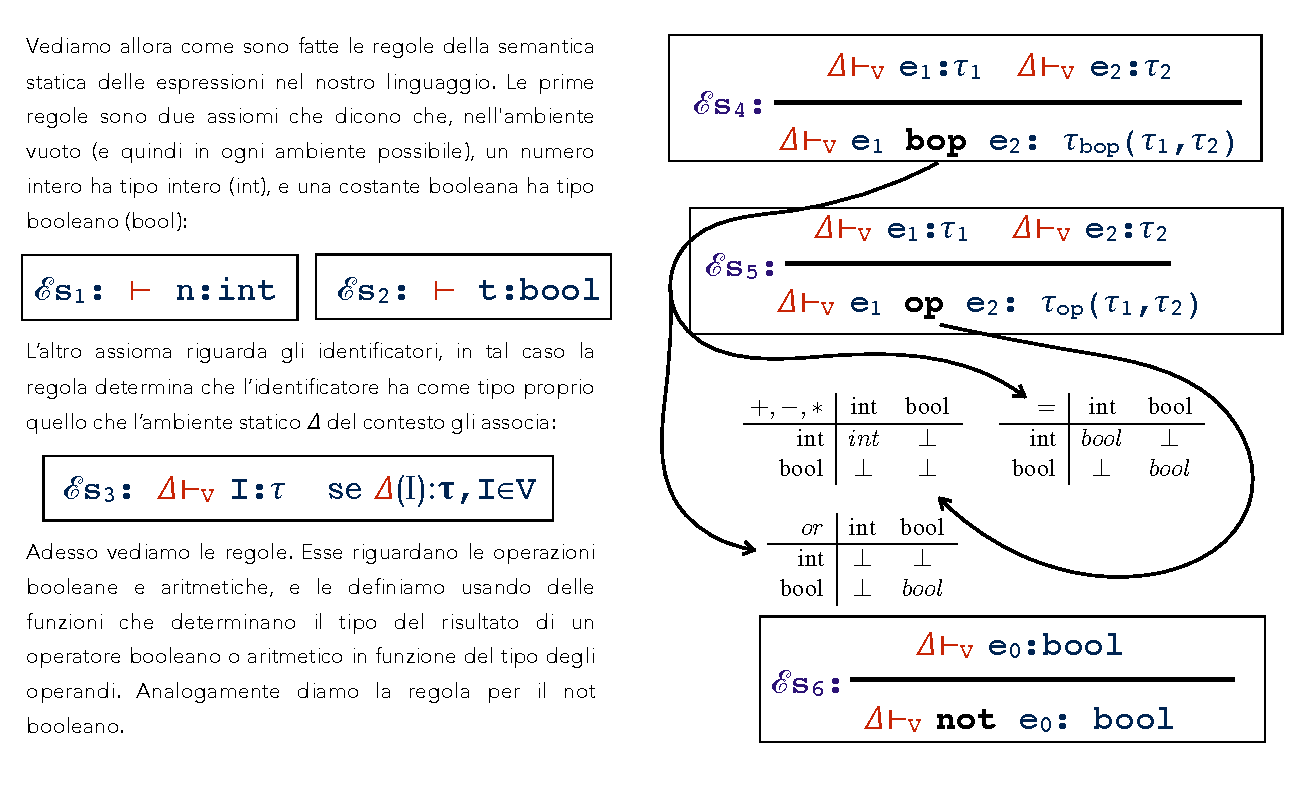
\includegraphics[scale=0.8]{1.pdf}
\end{center}

\paragraph*{Compatibilità d'ambiente} L'ambiente dinamico $\rho$ e l'ambiente dinamico $\Delta$ sono compatibili se 
\begin{align*}
\forall id \in I \hspace{0.3cm}(\Delta(I) = \tau) \text{ and } \rho(I) \in \tau \text{(valore di tipo $\tau$)}]
\end{align*}

\subsubsection*{regole definitive}
\begin{center}
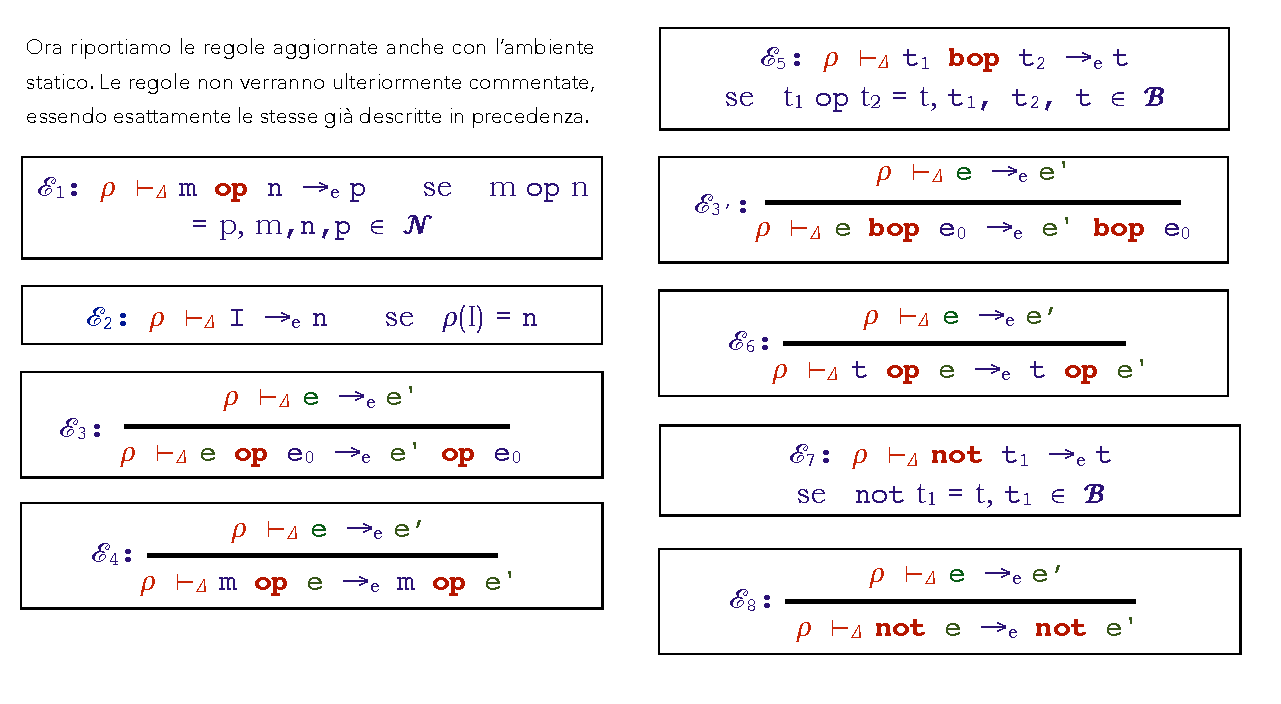
\includegraphics[scale=0.8]{2.pdf}
\end{center}

FINIRE

\end{document}